\documentclass{article}
\usepackage{import}
\usepackage{amsmath}
\usepackage{float}
\usepackage[utf8]{inputenc}
\usepackage{graphicx}
\usepackage{setspace}
\usepackage{geometry}
\usepackage{enumitem}
\usepackage{multirow}
\usepackage{tabularx}
\usepackage{array}
\usepackage{tocloft}
\usepackage{xcolor}
\geometry{a4paper, portrait, margin=30mm, bmargin=30mm, tmargin=30mm}
\setcounter{secnumdepth}{5}
\setcounter{tocdepth}{5}

\makeatletter
\newcommand\subsubsubsection{\@startsection{paragraph}{4}{\z@}{-2.5ex\@plus -1ex \@minus -.25ex}{1.25ex \@plus .25ex}{\normalfont\normalsize\bfseries}}
\newcommand\subsubsubsubsection{\@startsection{subparagraph}{5}{\z@}{-2.5ex\@plus -1ex \@minus -.25ex}{1.25ex \@plus .25ex}{\normalfont\normalsize\bfseries}}
\makeatother


\begin{document}
\setstretch{1.5}
%\vspace{10mm}  % vertical space
\thispagestyle{empty}
% \addvspace{5mm}  % vertical space until length

%$$$$$$$$$$$$$$$$$$$$$$$$$$$$$$$$$$$$$$$$$$$$$$$$$$$$$$$$$$$$$$$$$$$$$$$$$$$$$$$$$

\newgeometry{top=0.6in, bottom=0.6in, left=0.6in, right=0.6in}
% Make the title page
\begin{titlepage}
    \begingroup % Start a local scope
    \renewcommand{\baselinestretch}{1.75}\normalsize 
    \begin{center}
        % Draw a border around the entire page
        \setlength{\fboxrule}{1pt} 
        \setlength{\fboxsep}{2pt} 
        \fbox{
            \begin{minipage}[c][0.98\textheight][c]{0.98\textwidth} % Adjust content width
                \centering
                \vspace{-30mm} % Reduce vertical space at the top
                % University name and department
                \makebox[\textwidth][c]{\normalsize \textbf {UNIVERSITY OF SCIENCE AND TECHNOLOGY OF HANOI}} \\[5pt]
                \makebox[\textwidth][c]{\normalsize \textbf {DEPARTMENT OF INFORMATION AND COMMUNICATION TECHNOLOGY}} \\[20pt]
            
                % USTH logo
                
\includegraphics[width=0.5\textwidth]{image/usth.png} \\[15pt]
            
                % Report title
                \textbf{\LARGE GROUP PROJECT REPORT} \\[3pt]
                \textbf{\fontsize{19}{22}\selectfont USTH Connect}\\
                \textbf{\fontsize{19}{22}\selectfont Integrated app for university life assistant \\ and student networking} \\[30pt]
            
                % Group members section
                \textbf{\large Group Members} \\[10pt]
                \begin{tabular}{l@{\hskip 3cm}l} % Add spacing of 3cm between columns
                Nguyen Thi Van    & 22BI13459 \\
                Chu Hoang Viet     & 22BI13462 \\
                Nguyen Hoai Anh        & 22BI13021 \\
                Nguyen Dang Nguyen & 22BI13340 \\
                Do Minh Quang           & 22BI13379 \\
                \end{tabular} \\[20pt]
            
                % Supervisor section
                \textbf{\large Supervisor} \\[3pt]
                Assoc. Prof. Tran Giang Son \\[20pt]
            
                % Footer
                \textbf{January, 2025}
            \end{minipage}
        }
    \end{center}
    \endgroup % End local scope
\end{titlepage}

% Restore margins for the rest of the document
\restoregeometry

\thispagestyle{empty}

% end of title page
%$$$$$$$$$$$$$$$$$$$$$$$$$$$$$$$$$$$$$$$$$$$$$$$$$$$$$$$$$$$$$$$$$$$$$$$$$$$$$$$$$
\newpage

\renewcommand{\listfigurename}{LIST OF FIGURES}
\renewcommand{\cftloftitlefont}{\Large\bfseries} 
\renewcommand{\cftafterloftitle}{
    \par\noindent\vspace{-0.5em}
    \textcolor{blue}{\rule{\textwidth}{0.5pt}}
    \vspace{1em} 
}
\renewcommand{\cftfigpresnum}{Figure~}
\renewcommand{\cftfigaftersnum}{:}
\setlength{\cftfignumwidth}{5em}

\tableofcontents
\newpage

\listoffigures
\renewcommand{\listtablename}{LIST OF TABLES}
\renewcommand{\cftlottitlefont}{\Large\bfseries} 
\renewcommand{\cftafterlottitle}{
    \par\noindent\vspace{-0.5em}
    \textcolor{blue}{\rule{\textwidth}{0.5pt}}
    \vspace{1em} 
}
\renewcommand{\cfttabpresnum}{Table~}
\renewcommand{\cfttabaftersnum}{:}
\setlength{\cfttabnumwidth}{5em}
\newpage

\listoftables
\newpage



\section{Introduction}

\subsection{Context and Motivation}
University life often presents a wide range of challenges for both students and administrators. At USTH, managing academic schedules, building social connections, and navigating campus resources can become an irritated tasks.
The limitations of traditional systems, which are sometimes inconvenient, fragmented, and unable to kept track of, only add to the complexity.
These systems find it hard to provide up-to-date information and lack of integration needed to offer a seamless experience for students, which leaves a feeling of overwhelmed and disconnected for student.

To overcome these challenges, we developed USTH Connect, an integrated University Life Assistant and Student Networking Application.
USTH Connect combines advanced technologies like Spring Boot for backend services, Google Calendar for managing schedule, MapBox for campus navigation, and Moodle for accessing academic resources. Additionally, it employs Machine Learning to power its StudyBuddy feature, which allows students to connect with peers who share similar academic interests and goals.

USTH Connect is desgined to simplify academic and campus life. It combines all key resources into a user-friendly Android application, offering easy access to class schedules, course materials, and campus navigation tools.
Apart from academic, the platform encourages more connections between students, especially the first year student, making it easier to build meaningful relationships and collaborate effectively. 
With StudyBuddy, students can find compatible study partners, chat, and even make audio calls through secure VoIP functionality powered by Linphone.

USTH Connect places a strong emphasis on data security and system reliability. It utilizes a secure PostgreSQL database to manage data centrally, ensuring both protection and efficiency.
Additionally, communication between the backend and mobile devices is secured through the Tailscale VPN, providing strong protection for student privacy and uniterrupted access to the platform's features.

This report explores the design and development of USTH Connect, detailing the project's workflow, main features, and the challenges faced during its implementation. 
It also highlights the creative solutions used to address these challenges, demonstrating how USTH Connect enhances the university experience for students, faculty, and administrators.

\subsection{Project Objectives}
The primary objective of this project is to design, develop and implement an integrated system that enhances
university life and fosters student networking through advanced technological solutions.
The goal is to create a platform that seamlessly intergrates personal academic data, event annoucements, and campus resources.
By using advanced frameworks and APIs, together with recommendation system, we aim to simplify the administrative tasks, improve campus accessibility, 
and encourage more interaction among students.
This platform should be user-friendly and accessible through all devices, making it easier for students to experience campus life, 
stay informed, and connect with their peers. 

\subsection{Desired Outcomes}

\subsection{Structure of Thesis}
The thesis will be structured as follows:
\begin{itemize}
    \item \textbf{Part I: Introduction }
    \newline
    Provide a general introduction to the thesis, including an overview of the project, its objectives, and the scope of the work.
    \item \textbf{Part II: Requirement Analysis }
    \newline
    Lists all the tools, techniques, and system requirements used in the project. It includes
    both functional and non-functional requirements, as well as desired functionalities.
    \item \textbf{Part III: Methodologies }
    \newline
    System architecture, database design, and implementation details of various features, illustrated with sequence diagrams.
    \item \textbf{Part IV: AI Model Analysis and Training }
    \newline
    Analysis and training of AI models for recommend system for study buddy matchmaking, including datasets and model development, with (Model Name) integration.
    \item \textbf{Part V: Results and Discussions }
    \newline 
    Summarizes the implementations and achievements of the system. It reflects on how the
    objectives were met and provides a summary of the project's outcomes.
    \item \textbf{Part VI: Conclusion and Future Work }
    \newline
\end{itemize}


\subsection{Related works}

In this part we will cite some related works/papers that we used mainly for this 
project. We also summarize the content of these resources.


% \section{Theoretical Background}
\section{Requirement Analysis}
\subsection{System requirements}
\subsubsection{Functional Requirements}
\subsubsection{Non-functional Requirements}
\subsubsection{Desired Functionalities}

\subsection{Use Case}
\subsubsection{Use Cases Diagram}
    The below diagram is to demonstrate the interaction between users and system:
    % Figure
\subsubsection{Use Case Characteristics}
    The system in Figure above has two roles: \textbf{Admin} and \textbf{Student}:
    \begin{itemize}
        \item \textbf{Admin:} Admins have access to all students' functionalities. 
        Additionally, they can manage schedules, campus, resources and create and manage student accounts.
        \item \textbf{Student:}  Students can login, reset their password. They have permission to check their schedule, university campus and resources. Additionally, they can connect to other students, who share the same interests, subjects, hobbies,  by using StudyBuddy.
    \end{itemize}

\subsection{Use Case and Scenario Description}
    This section provides a detailed description of the various use cases and scenarios within the USTH Connect application. 
    Each use case outlines the interactions between students and the system, describing how the system responds to specific student actions.
\subsubsection{Use case: Authenticate}
    \begin{figure}[H]
        \centering
        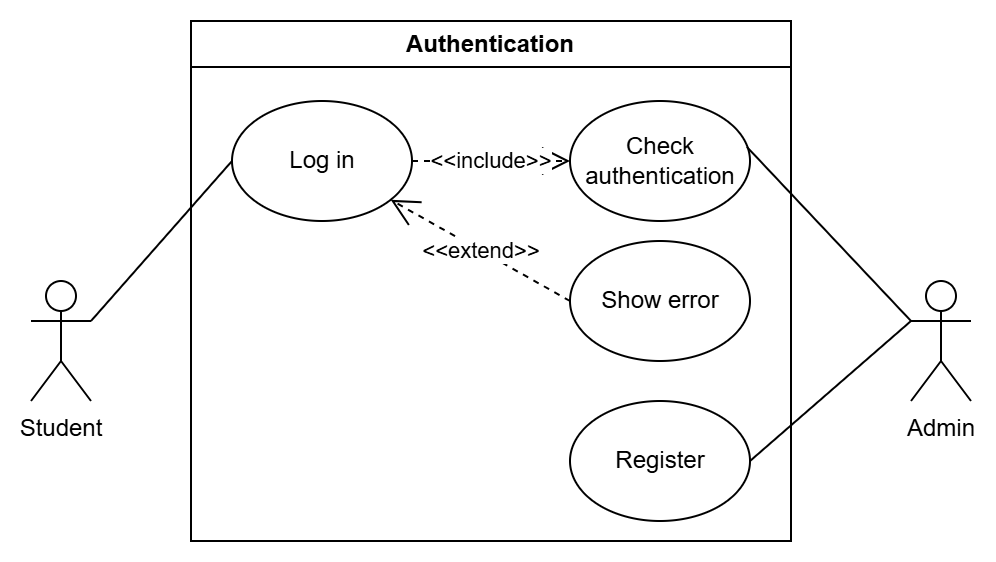
\includegraphics[width=0.7\textwidth]{image/AuthenticationUseCase.png} 
        \caption{Authentication use case diagram}
        \label{fig:authenticate_use_case}
    \end{figure}
    \textbf{Description:} Students can login and reset their passwords in case they forget them. Admin has to create accounts for students.

    \noindent \textbf{Pre-conditions:} Before this use case begins, students must ensure that all system packages are fully installed to avoid errors.

    \noindent \textbf{Post-conditions:}
    \begin{itemize}
        \item \textbf{Success:} Students can access the main screen.
        \item \textbf{Failure:} Not displaying the main screen, error message is shown in the system.
    \end{itemize}

    
    \begin{table}[H]
        \centering
        \renewcommand{\arraystretch}{1.5}
        \caption{Actor Actions and System Actions for Authenticate}
        \label{tab:authenticate_table}
        \begin{tabular}{|m{3.5cm}|p{10cm}|} 
            \hline
            \multicolumn{1}{|c|}{\textbf{Actor Action}} & \multicolumn{1}{c|}{\textbf{System Action}} \\ \hline
            & 1. Students enter studentID and password given by Admin \\ \cline{2-2} 
            \multirow{4}{=}{\centering \shortstack[c]{Login to the system \\ (User)}} 
            & 2. System verifies studentID and password against the stored database \\ \cline{2-2}
            & 3. If both studentID and password are correct, the system grants access to the student and displays the main screen \\ \cline{2-2}
            & 4. If it is incorrect, the system displays an error message and asks students to re-enter \\ \hline
            & 1. Student enters studentID and old password \\ \cline{2-2}
            \multirow{5}{=}{\centering \shortstack[c]{Change Password \\ (User)}} 
            & 2. System verifies studentID and password against the stored database \\ \cline{2-2}
            & 3. If the information entered is correct, students can change their password \\ \cline{2-2}
            & 4. System updates the new password in the database \\ \cline{2-2}
            & 5. Students enter the new password to login \\ \hline
        \end{tabular}
    \end{table}
    
    

\subsubsection{Use case: Student Schedule}
    \begin{figure}[H]
        \centering
        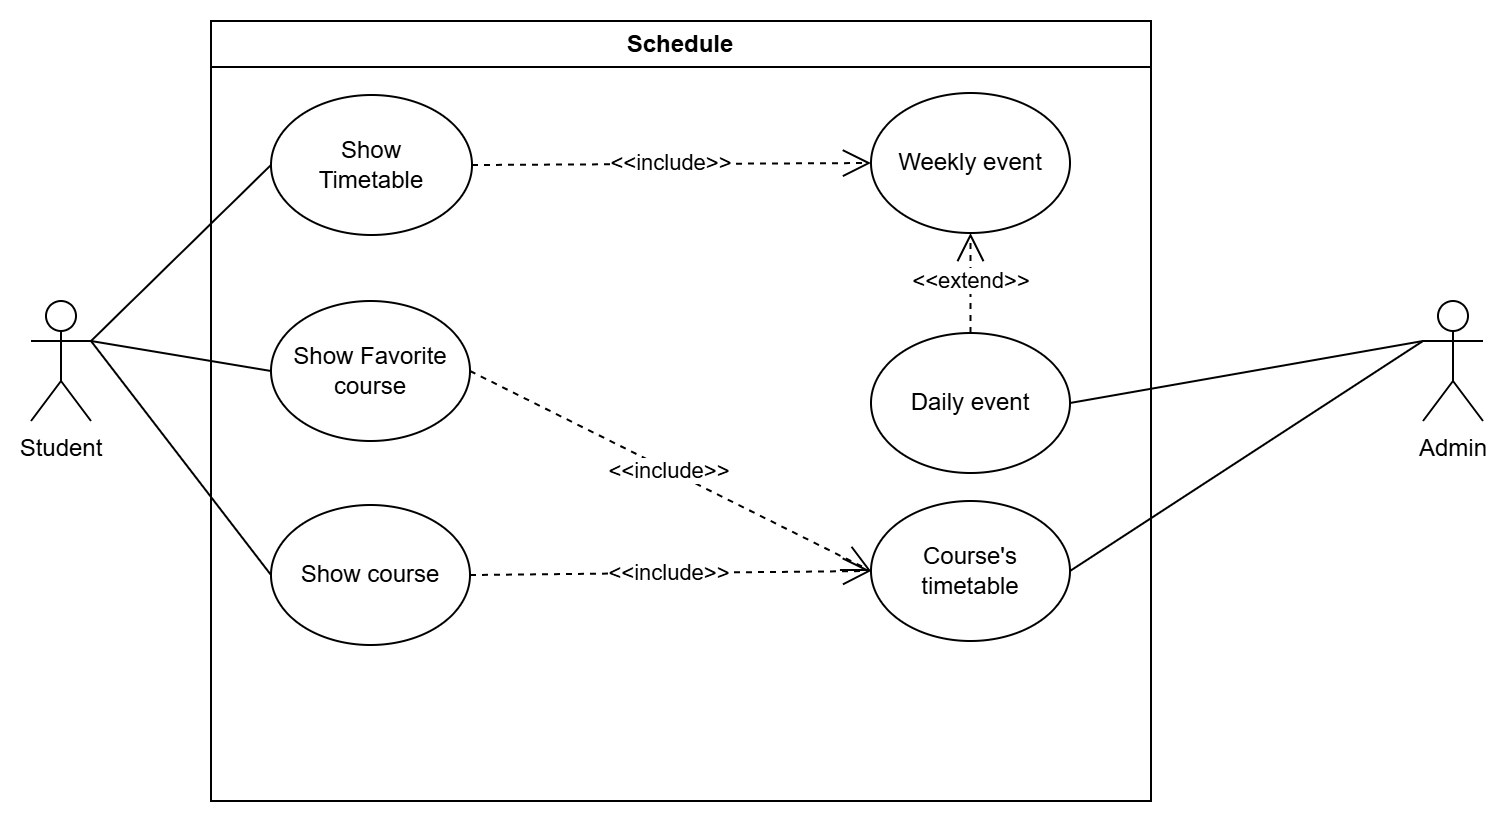
\includegraphics[width=0.7\textwidth]{image/StudentScheduleUseCase.drawio.png} 
        \caption{Schedule use case diagram}
        \label{fig:schedule_use_case}
    \end{figure}
    \textbf{Description:} This use case enables students to view their academic timetable. The system sync schedule every 10 minutes to make sure no daily event is missing.

    \noindent \textbf{Pre-conditions:} 
        \begin{itemize}
            \item Before this use case begins, students must be logged into the system.
            \item The system up-to-date course details: time, locations, lecturer.
        \end{itemize}
    \noindent \textbf{Post-conditions:}
    \begin{itemize}
        \item \textbf{Success:} 
        \begin{itemize}
            \item Students can see their daily events.
            \item System sends notification if there is a new class or a canceled class.
        \end{itemize}
        \item \textbf{Failure:} Not display the event daily and show error messages.
    \end{itemize}

    \begin{table}[H]
        \centering
        \renewcommand{\arraystretch}{1.5}
        \caption{Actor Actions and System Actions for Schedule}
        \label{tab:schedule_table}
        \begin{tabular}{|m{3.5cm}|p{10cm}|} 
            \hline
            \multicolumn{1}{|c|}{\textbf{Actor Action}} & \multicolumn{1}{c|}{\textbf{System Action}} \\ \hline
            \multirow{3}{=}{\centering \shortstack[c]{User click button \\ "Timetable"}} 
            & 1. The system shows a calendar \\ \cline{2-2} 
            & 2. Students can change the day, week, month format in the calendar \\ \cline{2-2}
            & 3. After choosing a day, students can see daily events \\ \hline
            \multirow{3}{=}{\centering \shortstack[c]{User click button \\ "Favorite Course"}} 
            & 1. The system shows a list of favorite courses which are added by Students \\ \cline{2-2}
            & 2. Students can see the timetable of their favorite course after clicking it \\ \cline{2-2}
            & 3. Un-click the favorite icon, the system will delete that course out of the list of favorite courses \\ \hline
            \multirow{3}{=}{\centering \shortstack[c]{User click button \\ "Course"}} 
            & 1. The system shows all the courses which match with the student’s major and year \\ \cline{2-2}
            & 2. Students can see the course class timetable after clicking the course \\ \cline{2-2}
            & 3. Click the favorite icon, the system will add that course to the list of favorite courses and show them in Favorite Course \\ \hline
        \end{tabular}
    \end{table}

\subsubsection{Use case: University Campus}
    \begin{figure}[H]
        \centering
        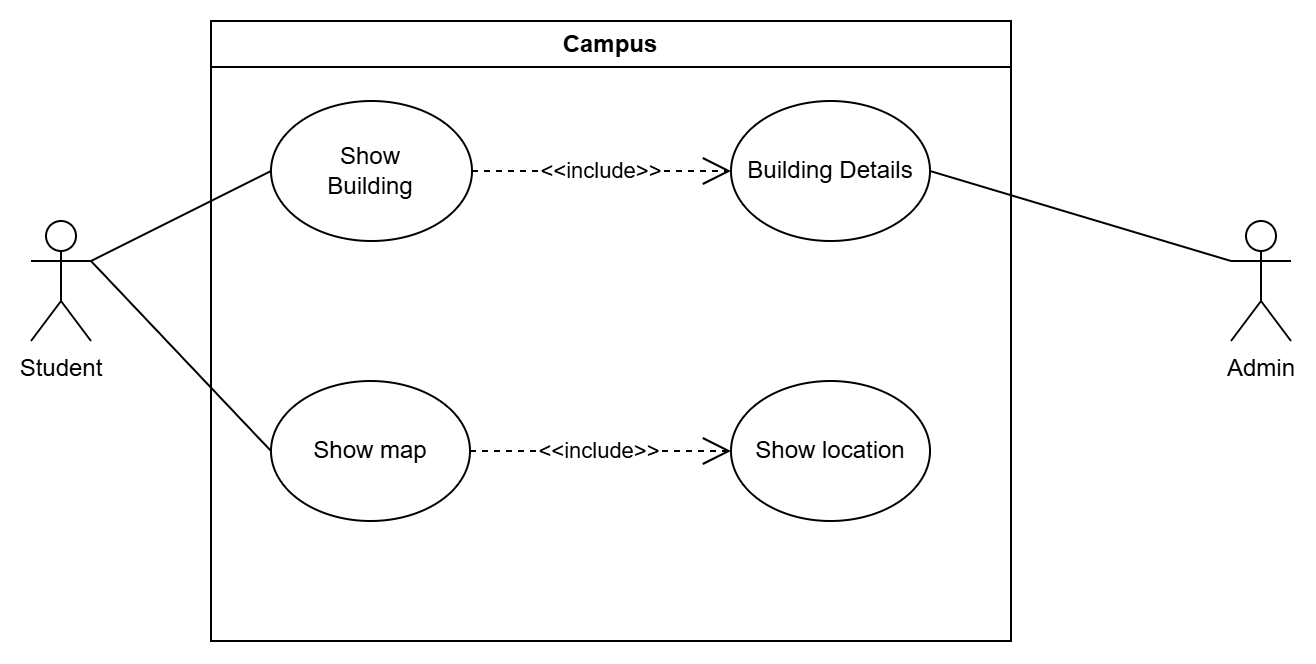
\includegraphics[width=0.7\textwidth]{image/CampusUseCase.png} 
        \caption{Campus use case diagram}
        \label{fig:campus_use_case}
    \end{figure}
    \textbf{Description:} The system displays a list of campus buildings and their details. The system can locate each building in a list on a map.

    \noindent \textbf{Pre-conditions:} 
        \begin{itemize}
            \item Before this use case begins, students must be logged into the system.
            \item Building data must be fetched from the database.
        \end{itemize}
    \noindent \textbf{Post-conditions:}
    \begin{itemize}
        \item \textbf{Success:} 
        \begin{itemize}
            \item Students can search for buildings on campus and each details.
            \item System shows a map where the student and building are located.
        \end{itemize}
        \item \textbf{Failure:} The system displays an error message or map fails to load.
    \end{itemize}

    \begin{table}[H]
        \centering
        \renewcommand{\arraystretch}{2.5}
        \caption{Actor Actions and System Actions for Campus}
        \label{tab:campus_table}
        \begin{tabular}{|m{3.5cm}|p{10cm}|} 
            \hline
            \multicolumn{1}{|c|}{\textbf{Actor Action}} & \multicolumn{1}{c|}{\textbf{System Action}} \\ \hline
            \multirow{2}{=}{\centering \shortstack[c]{User click button \\ "Building"}} 
            & 1. The system shows a list of buildings which students study in \\ \cline{2-2} 
            & 2. After clicking a building, the system returns its details \\ \hline
            \multirow{1}{=}{\centering \shortstack[c]{User click button \\ "Map"}} 
            & 1. System loads a map to locate your location and each building \\ \hline
        \end{tabular}
    \end{table}

\subsubsection{Use case: University Resource}
    \textbf{Description:} Students can access lectures, slides, exercises and homework from all bachelor’s programs, which the system displays.

    \noindent \textbf{Pre-conditions:} 
        \begin{itemize}
            \item Before this use case begins, students must be logged into the system.
            \item Lectures, slides, exes and homeworks must be fetched successfully.
        \end{itemize}
    \noindent \textbf{Post-conditions:}
    \begin{itemize}
        \item \textbf{Success:} Students can access and download all resources from all bachelor’s programs.
        \item \textbf{Failure:} The system displays an error message or resource fail to open or fail to load data.
    \end{itemize}

    \begin{table}[H]
        \centering
        \renewcommand{\arraystretch}{2.5}
        \caption{Actor Actions and System Actions for Resource}
        \label{tab:resource_table}
        \begin{tabular}{|m{3.5cm}|p{10cm}|} 
            \hline
            \multicolumn{1}{|c|}{\textbf{Actor Action}} & \multicolumn{1}{c|}{\textbf{System Action}} \\ \hline
            \multirow{2}{=}{\centering \shortstack[c]{User click button \\ "Show Resource"}} 
            & 1. The system displays a list of bachelor’s programs \\ \cline{2-2} 
            & 2. After choosing bachelor’s programs, the screen shows majors, then, the system shows the subject of the major and lectures, slides, … of a subject of major \\ \hline
        \end{tabular}
    \end{table}

\subsubsection{Use case: Student StudyBuddy}
    \begin{figure}[H]
        \centering
        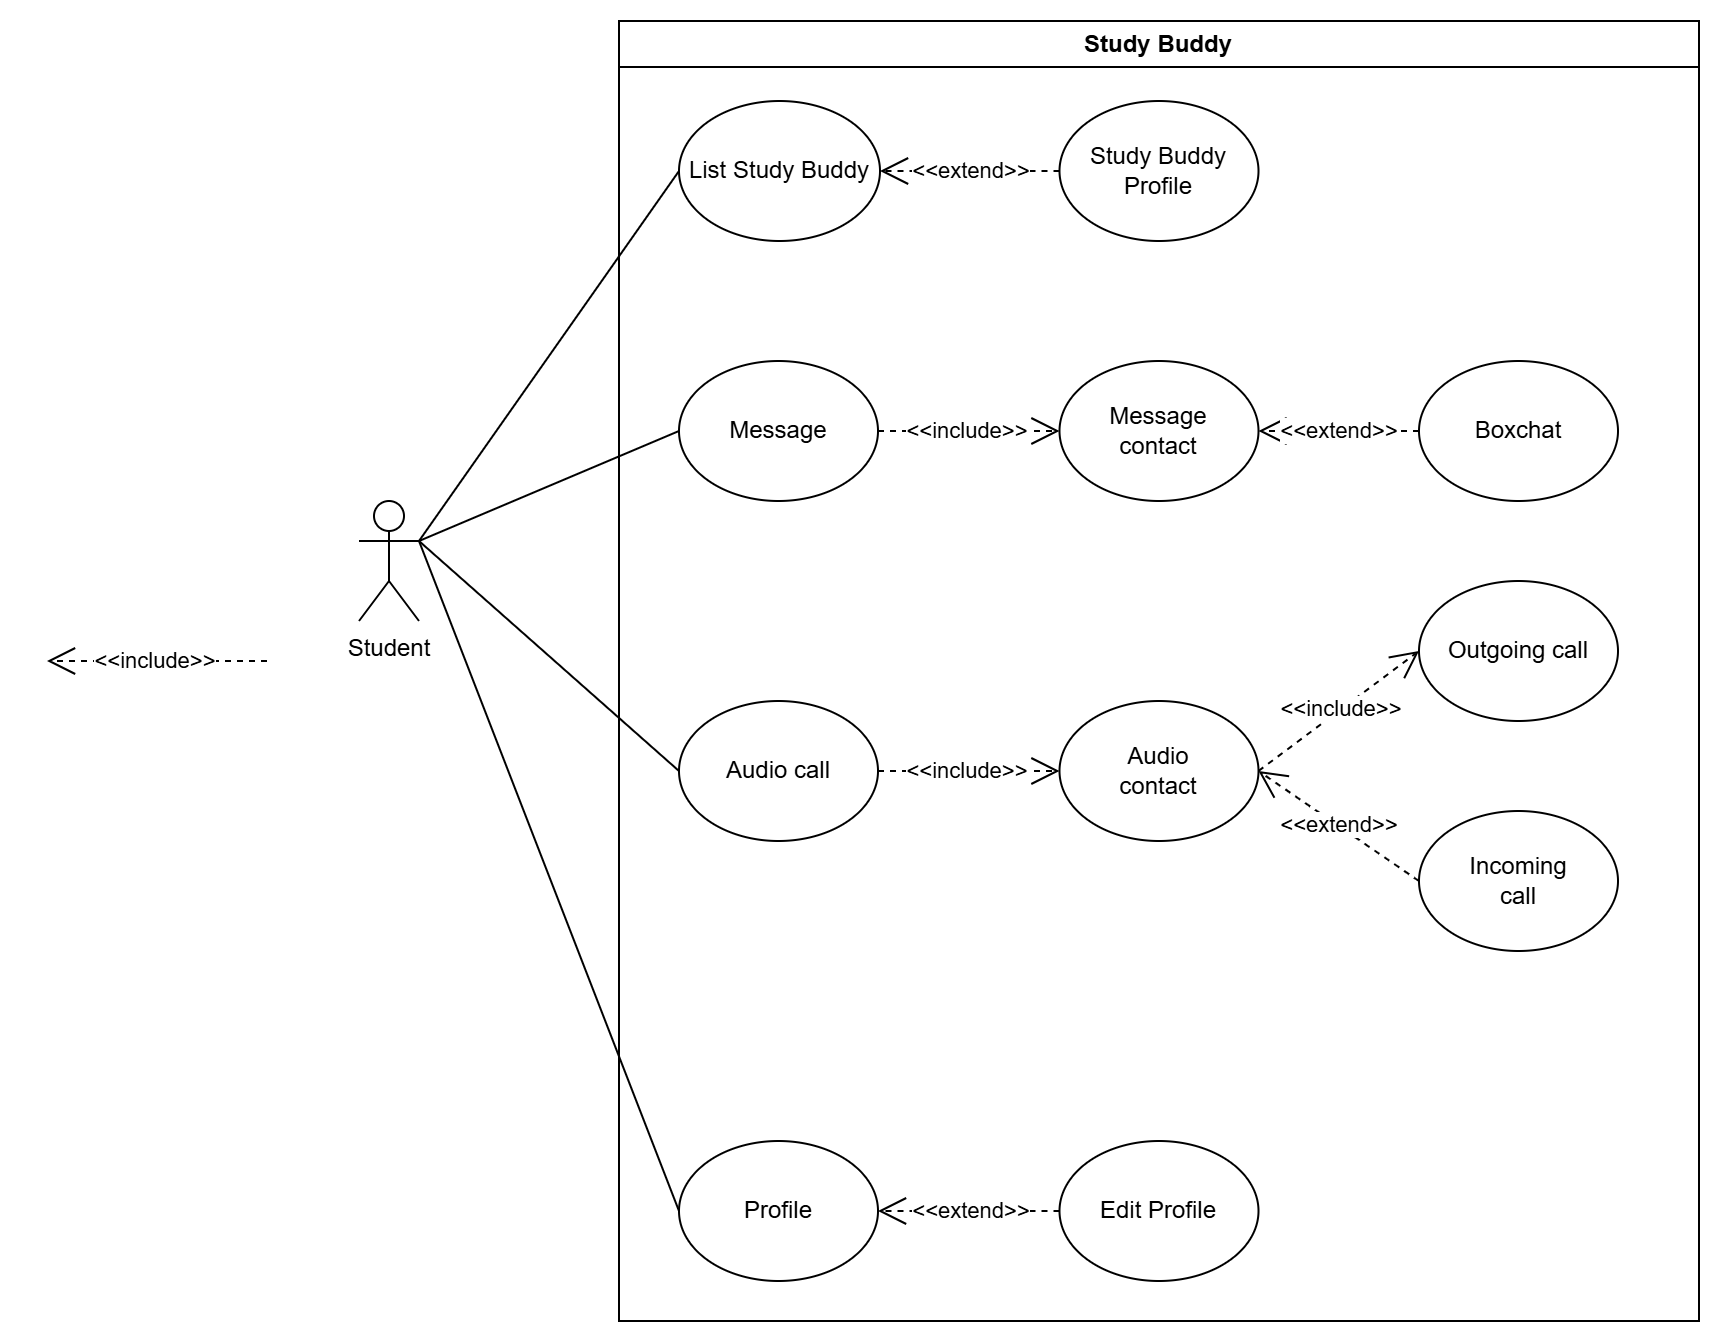
\includegraphics[width=0.7\textwidth]{image/StudyBuddyUseCase.png} 
        \caption{StudyBuddy use case diagram}
        \label{fig:studyBuddy_use_case}
    \end{figure}
    \textbf{Description:} The system allows students to connect and find each other students, who have the same things with the other. Students can view their profile, interest, ...

    \noindent \textbf{Pre-conditions:} 
        \begin{itemize}
            \item Before this use case begins, students must do a small survey and be logged into the system.
            \item The system must fetch successfully with other students’ profiles.
        \end{itemize}
    \noindent \textbf{Post-conditions:}
    \begin{itemize}
        \item \textbf{Success:}
        \begin{itemize}
            \item User can view a list of suggestion friends; send and receive text message, audio call; view and update profile.
            \item Admins can refresh and reload the suggestion matching list.
        \end{itemize}
        \item \textbf{Failure:}
        \begin{itemize}
            \item The system fails to fetch student data.
            \item System fails to displayprofile of match recommendation.
            \item System display an error message. 
        \end{itemize}
    \end{itemize}

    \begin{table}[H]
        \centering
        \renewcommand{\arraystretch}{1.5}
        \caption{Actor Actions and System Actions for StudyBuddy}
        \label{tab:studyBuddy_table}
        \begin{tabular}{|m{3.5cm}|p{10cm}|} 
            \hline
            \multicolumn{1}{|c|}{\textbf{Actor Action}} & \multicolumn{1}{c|}{\textbf{System Action}} \\ \hline
            \multirow{4}{=}{\centering \shortstack[c]{User click button \\ "StudyBuddy"}} 
            & 1. The system displays a list of Students who are in the list of recommendations \\ \cline{2-2} 
            & 2. After clicking the “Yes” button, add that Student to Chat and Contact \\ \cline{2-2}
            & 3. After clicking the “No” button, remove that Student from the list \\ \cline{2-2}
            & 4. After clicking the “Refresh” button, the system will refresh the list of recommended students \\ \hline
            \multirow{2}{=}{\centering \shortstack[c]{User click button \\ "Message"}} 
            & 1. The system displays students who Students have matched with \\ \cline{2-2}
            & 2. After clicking the box chat, start a chat with another student \\ \hline
            \multirow{2}{=}{\centering \shortstack[c]{User click button \\ "Contact"}} 
            & 1. The system displays students who Students have matched with \\ \cline{2-2}
            & 2. After clicking the contact, start an audio call with another student \\ \hline
            \multirow{2}{=}{\centering \shortstack[c]{User click button \\ "Profile"}} 
            & 1. The system fetches the StudyBuddy profile of Student from the database \\ \cline{2-2}
            & 2. After clicking “Edit Profile”, Students can change information about their StudyBuddy profile after the system is verified \\ \hline
        \end{tabular}
    \end{table}

\subsubsection{Use case: Real Time Notification}
    \begin{figure}[H]
        \centering
        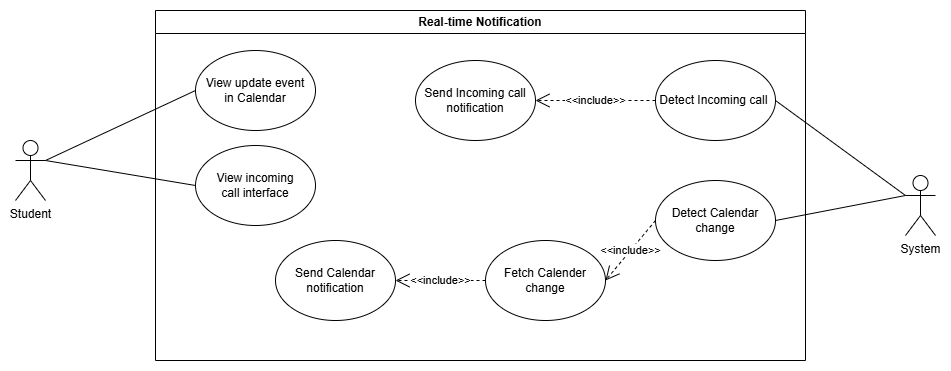
\includegraphics[width=0.7\textwidth]{image/Real-timeNotificationUseCase.png} 
        \caption{Real Time Notification use case diagram}
        \label{fig:notification_usecase}
    \end{figure}
    \textbf{Description:} The push notification system alerts the user whenever there is a change in their calendar (a new event or modification of an existing one) or when they receive a call. Notifications are delivered in real-time, ensuring that the user stays updated on any important events or incoming calls. 
    
    \noindent \textbf{Pre-conditions:} 
        \begin{itemize}
            \item The user’s device must be connected to the internet.
            \item The user must have granted the application permission to access the calendar and incoming notifications.
        \end{itemize}
    \noindent \textbf{Post-conditions:}
    \begin{itemize}
        \item The real time notification will pop up on the user's device to attract the user's attention.
        \item The notifications will contain:
        \begin{itemize}
            \item A bolded title with context about the notification’s content.
            \item The application icon to show where the notification is coming from.
            \item A subtext for describing more information about the notification.
        \end{itemize}
    \end{itemize}

    \begin{table}[H]
        \centering
        \renewcommand{\arraystretch}{1.5}
        \caption{Actor Actions and System Actions for Real time Notification}
        \label{tab:notification_table}
        \begin{tabular}{|m{3.5cm}|p{10cm}|} 
            \hline
            \multicolumn{1}{|c|}{\textbf{Actor Action}} & \multicolumn{1}{c|}{\textbf{System Action}} \\ \hline
            \multirow{2}{=}{\centering \shortstack[c]{Admin update or \\ add event to \\ the user’s calendar}} 
            & 1. The system detects the calendar changes and triggers the notification \\
            & \\ \hline 
            \multirow{2}{=}{\centering \shortstack[c]{User receives \\ an incoming call}} 
            & 1. The system identifies incoming calls and sends a push notification to inform users in real time \\ \hline
            \multirow{2}{=}{\centering \shortstack[c]{User click on \\ the notification}} 
            & 1. \textbf{Calendar notification:} The system will open the application and display the updated event on the calendar \\ \cline{2-2}
            & 2. \textbf{Incoming call notification:} The system will open the application and allow the user to handle the incoming call (accept or decline) \\ \hline
        \end{tabular}
    \end{table}


% \subsection{Mobile Application Background}
% In this part we will introduce about the standard mobile application framework.
% \subsubsection{Mobile Application Development}
% \subsubsubsection{Android Development Frameworks}
% For Android application development, Android Studio is considered as the primary Integrated Development Environment (IDE) for app development.
% According to Google, it is recommended as an ideal IDE for Android development and have a variety of powerful features including:
% \begin{itemize}
%     \item \textbf{XML (Extensible Markup Language) Layout Desgin:} Android Studio offers a visual layout editor for designing user interface (UI). 
%     XML seperates the UI design from business logic, enabling multiple designers and developers to work independently. XML layouts follow a tree structure where each elements will represent a UI component.
%     Each elements will have multiple attributes (layout, styles, ID,...) and layout types (ConstraintLayout, LinearLayout,...) to help implement an eye-catching and simple UI.
%     Moreover, by binding directly the layout components to corresponding properties in the code or transforming XML into runtime object using Layout Inflation.
%     \item \textbf{Gradle Build System: } In Android Studio, Gradle will take responsibility for automatic project building and management. 
%     It will handle requirement dependencies, compiled resources, and the most important is generating
%     \item 
% \end{itemize} 
% \subsubsubsection{UI/UX Design Principles}

% \subsubsubsection{Google Calendar Display}

% \subsubsubsection{MapBox Display}

% \subsubsubsection{Moodle Resource Display}

% \subsubsubsection{Real-Time Notifications}

% \subsubsubsection{Student Matching System}

% \subsubsection{Backend System}
% \subsubsubsection{Spring Boot Framework}

% \subsubsubsection{JWT and RBAC}

% \subsubsubsection{Database Management}

% \subsubsubsection{Google Calendar Integration}

% \subsubsubsection{MapBox Integration}

% \subsubsubsection{Moodle Integration}

% \subsubsubsection{Tailscale VPN}

% \subsubsubsection{Spring Boot Framework}
% \subsection{Machine Learning Background}
% In this part we will explain the theory and mathematical bases for
% the clustering algorithm that we used in this project.
% \begin{itemize} 
%     \item Machine Learning Workflow: describe a standard workflow for a clustering
%     algorithm.
%     \item Data encoding method: One Hot Encoding, Word Embedding TD-IDF
%     \item Dimensionality reduction
%     \item Clustering algorithm: K-mode (? can we use more algorithm for this part)
%     \item Evaluation Metrics: Silhouette score, Davies-Bouldin index

% \end{itemize}

\section{Methodologies}
\subsection{System Architecture}
\subsection{Database Design}
\subsection{Use Case Implementation}
\subsubsection{Sync Calendar Sequence Diagram}
\begin{figure}[H]
    \centering
    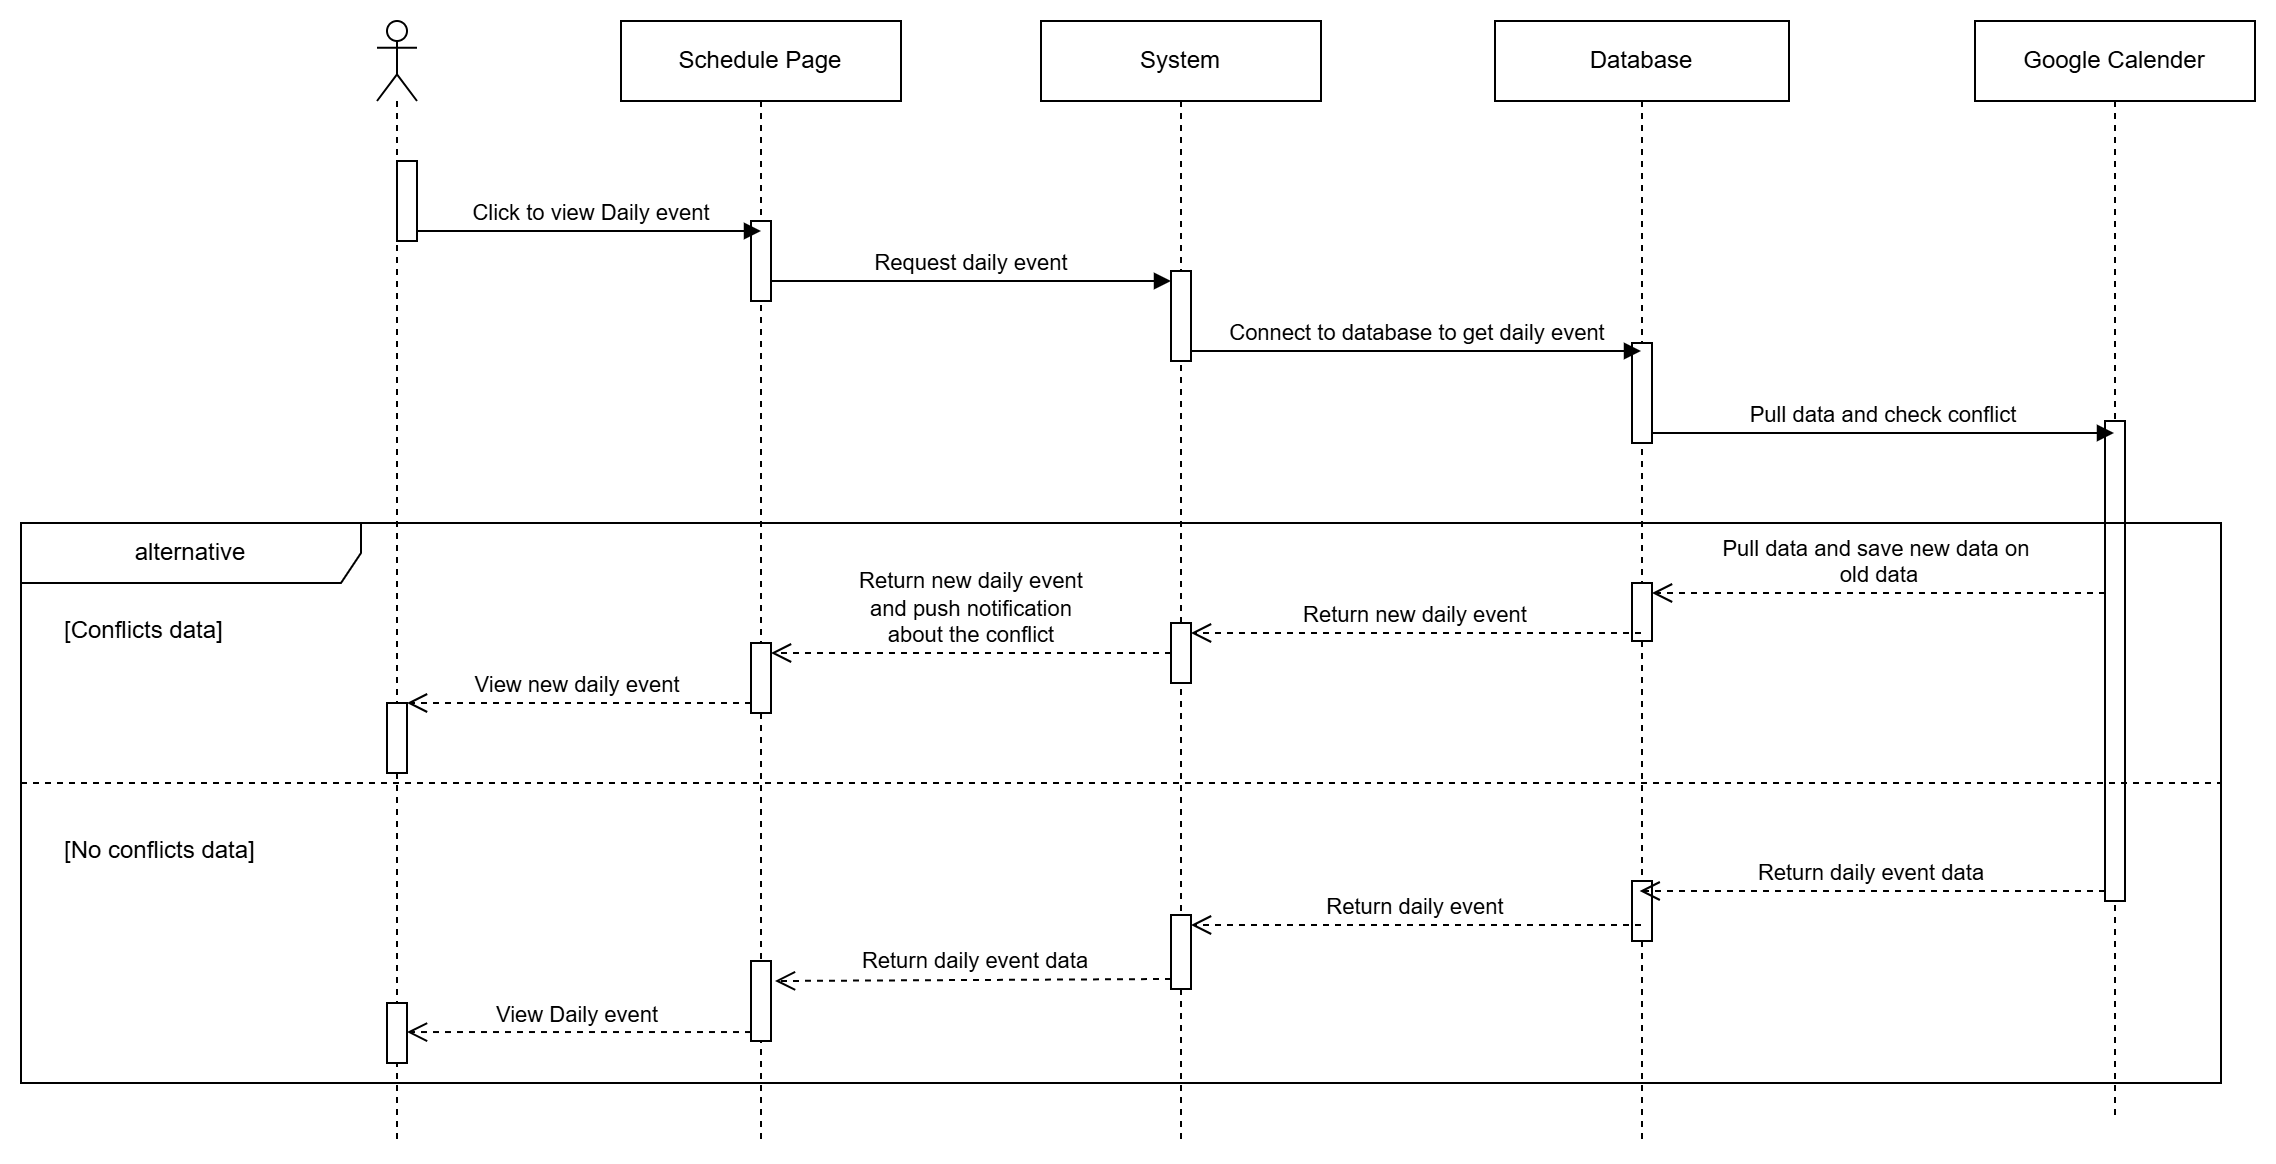
\includegraphics[width=1\textwidth, height=0.3\textheight]{image/SyncCalendar.png} 
    \caption{Synchronize Calendar sequence diagram}
    \label{fig:sync_calendar_sequence}
\end{figure}



\subsubsection{Analysis Call and Message Technologies}
\noindent This section below provides how the contact between users works utilising the help of SIP-based service Linphone.
\subsubsubsection{Session Initiation Protocol}

    In order to facilitate data exchange between two parties, 
    establishing a session is essential. However, identifying and connecting with 
    the second participant can be challenging. To address this, specialized protocols 
    have been designed specifically for such scenarios. \\

    \noindent The Session Initiation Protocol \cite{sip}, 
    commonly known as SIP, is a signaling protocol operating at the 
    application layer, designed for Internet telephony, IP-based telephone systems, 
    as well as mobile phone calling over LTE. SIP’s primary purpose is in VoIP systems, where it serves 
    as a support protocol for registering and locating users, and for call set up and management. It can initiate, maintain, 
    and terminate communication sessions that include voice, video and messaging applications. SIP supports five facets of establishing and terminating multimedia communications: 
    user location, user availability, user capabilities, session setup, and session management. \\

    \noindent SIP functions as a standalone application but relies on other protocols 
    to ensure the overall architecture operates effectively. At the transport layer, 
    it is transported by using the Transmission Control Protocol (TCP), the User Datagram Protocol (UDP), 
    or the Transport Layer Security (TLS) depending on specific circumstances. In this project, 
    TLS is used (more on TLS in Section 1.3). \\

    \noindent SIP architecture consists of:
    \begin{itemize}
        \item \textbf {User Agent (UA):} an end point of the network, able to send requests (also known as User Agent Client - UAC) 
        and receive responses (User Agent Server - UAS). User Agent usually acts as both client and server and some examples 
        are - IP phone, softphone, and camera. The caller’s phone acts as a client and the callee’s phone acts as a server.
        \item \textbf {The Proxy Server:} takes a request from a user agent and forwards it to another user (i.e., an INVITE message).
        \item \textbf {The Registrar Server:} which is responsible for registering users to the network. It accepts registration requests from 
        user agents and helps users to authenticate themselves within the network. It stores the URI and the location of users in a database 
        to help other SIP servers within the same domain.
        \item \textbf {The Redirect Server:} receives requests and looks up the intended recipient of the request in the location database created by the registrar. 
        \item \textbf {The Location Server:} provides information regarding the caller’s possible locations to the Redirect and Proxy Servers.
    \end{itemize}
    \noindent In SIP, Each user is identified with a unique address, called SIP Uniform Resource Identifier (SIP URI). It is an address that contains information for establishing a session with the other end. The SIP URI resembles an E-Mail address and is written in the syntax below with the following URI parameters: 
    SIP - URI = sip:x@y:Port  where x = username and y = host (domain or IP).

\subsubsubsection{Linphone}
    Linphone is an open-source VoIP (Voice over Internet Protocol) application that utilizes SIP-based user agent. VoIP messages and calls are made over an IP network rather than over traditional public switched telephone networks (PSTN). 
    Linphone features all basic SIP-related services, such as audio and video calls, call management, call transfer, audio conferencing, and instant messages. 
    
    \pagebreak

    The free Linphone SIP service is released with an open-source license; and the SIP server software powering this service is called Flexisip. 
    Linphone uses its open-source library as its core, called liblinphone. 
    The library is a SIP-based SDK5 for video and audio over IP and is written in C/C++. 
    The application is available on Linux, Windows, MacOS, iOS, and Android. \\

    \noindent The combination of Linphone and Flexisip SIP proxy provides secure end-user registration and call setup.
    More precisely, Linphone client establishes and maintains a SIP TLS connection to the Flexisip server. 
    The Linphone client verifies the SIP server’s identity based on the X.509 digital certificate of the server (a list of trusted root authorities is provided at compilation time). 
    In this way, message and entity authentication, as well as confidentiality, of the information exchanged between the Linphone client and the Flexisip server is ensured. 
\subsubsubsection{Transport Layer Security Protocol (TLS)}
    Transport Layer Security, or TLS, is a widely adopted security protocol designed to facilitate privacy and data security for communications over the Internet. 
    TLS was derived from a security protocol called Secure Socket Layer (SSL). A primary use case of TLS is encrypting the communication between applications and servers. 
    TLS is based on symmetric encryption and is a client - server model, where the client is able to authenticate the server and, optionally, the server is also able to authenticate the client. \\

    \noindent When using SIP over TLS, the whole SIP signalling is encrypted. However it holds only on the segments of the communication which actually use TLS. 
    Therefore, TLS will be automatically set to each end of the user by default in this project. 


\subsubsubsection{Communication Handling}
\subsubsubsubsection{Call Initialization}
    A session is initiated with an INVITE method which is the request from a UA client (caller). 
    INVITE has attributes containing source address, destination address, and information about the session from the caller. 
    The SIP client creates an INVITE message for callee, which is normally sent to a proxy server.

    \noindent If the OK message takes over 200ms to deliver, the progress and status (TRYING) are sent to the caller. 
    The three-way handshake occurs when the OK message confirms the connection to the caller and the ACK message confirms the existence of connection to the callee. 
    Then the media transport, which is logically separated from session initiation will be established. When there is a BYE message being sent, the session will be terminated. 

    \noindent The most common SIP messages explain for the above figure:
    \begin{itemize}
        \item \textbf {INVITE:} Initiate a dialog for establishing a call. The request is sent by a user agent client to a user agent server.
        \item \textbf {OK:} confirmation of a request.
        \item \textbf {ACK:} confirmation of the connection form caller to callee.
        \item \textbf{BYE:} Signal termination for a session and end a call.
    \end{itemize}

    \noindent Below is the illustration of a simple SIP operations:
    \begin{itemize}
        \item \textbf {Step 1:} SIP client creates INVITE message for callee, which is normally sent to a proxy server. The proxy server will then obtain the IP address of SIP server that handles requests for the requested domain. 
        \item \textbf {Step 2:} The proxy server will reference a location server to identify the next hop server. 
        \item \textbf {Step 3:} The location server (non - SIP server) stores information about the next hop server and will return the IP address of callee.
        \item \textbf {Step 4:} Trying message will be sent to the caller when the session initialization is in process.
        \item \textbf {Step 5:} When the IP address is achieved from the step 3, the proxy server will forward the INVITE message to callee machine.
        \item \textbf {Step 6 and 7:} The callee device will ring and the proxy server will forward the RINGING message from the callee to the caller.
        \item \textbf {Step 8 and 9:} When successfully reaching the callee, if the callee accepts the call, the OK response will be sent back from the callee to the caller through the proxy server.
        \item \textbf {Step 10:} An ACK confirmation will then be sent. After that a full-fledged media session is initiated between UAC and UAS. 
        \item \textbf {Step 11 and 12:} The session will then be terminated when one of two components sends the BYE message. 
    \end{itemize}

    \begin{figure}[H]
        \centering
        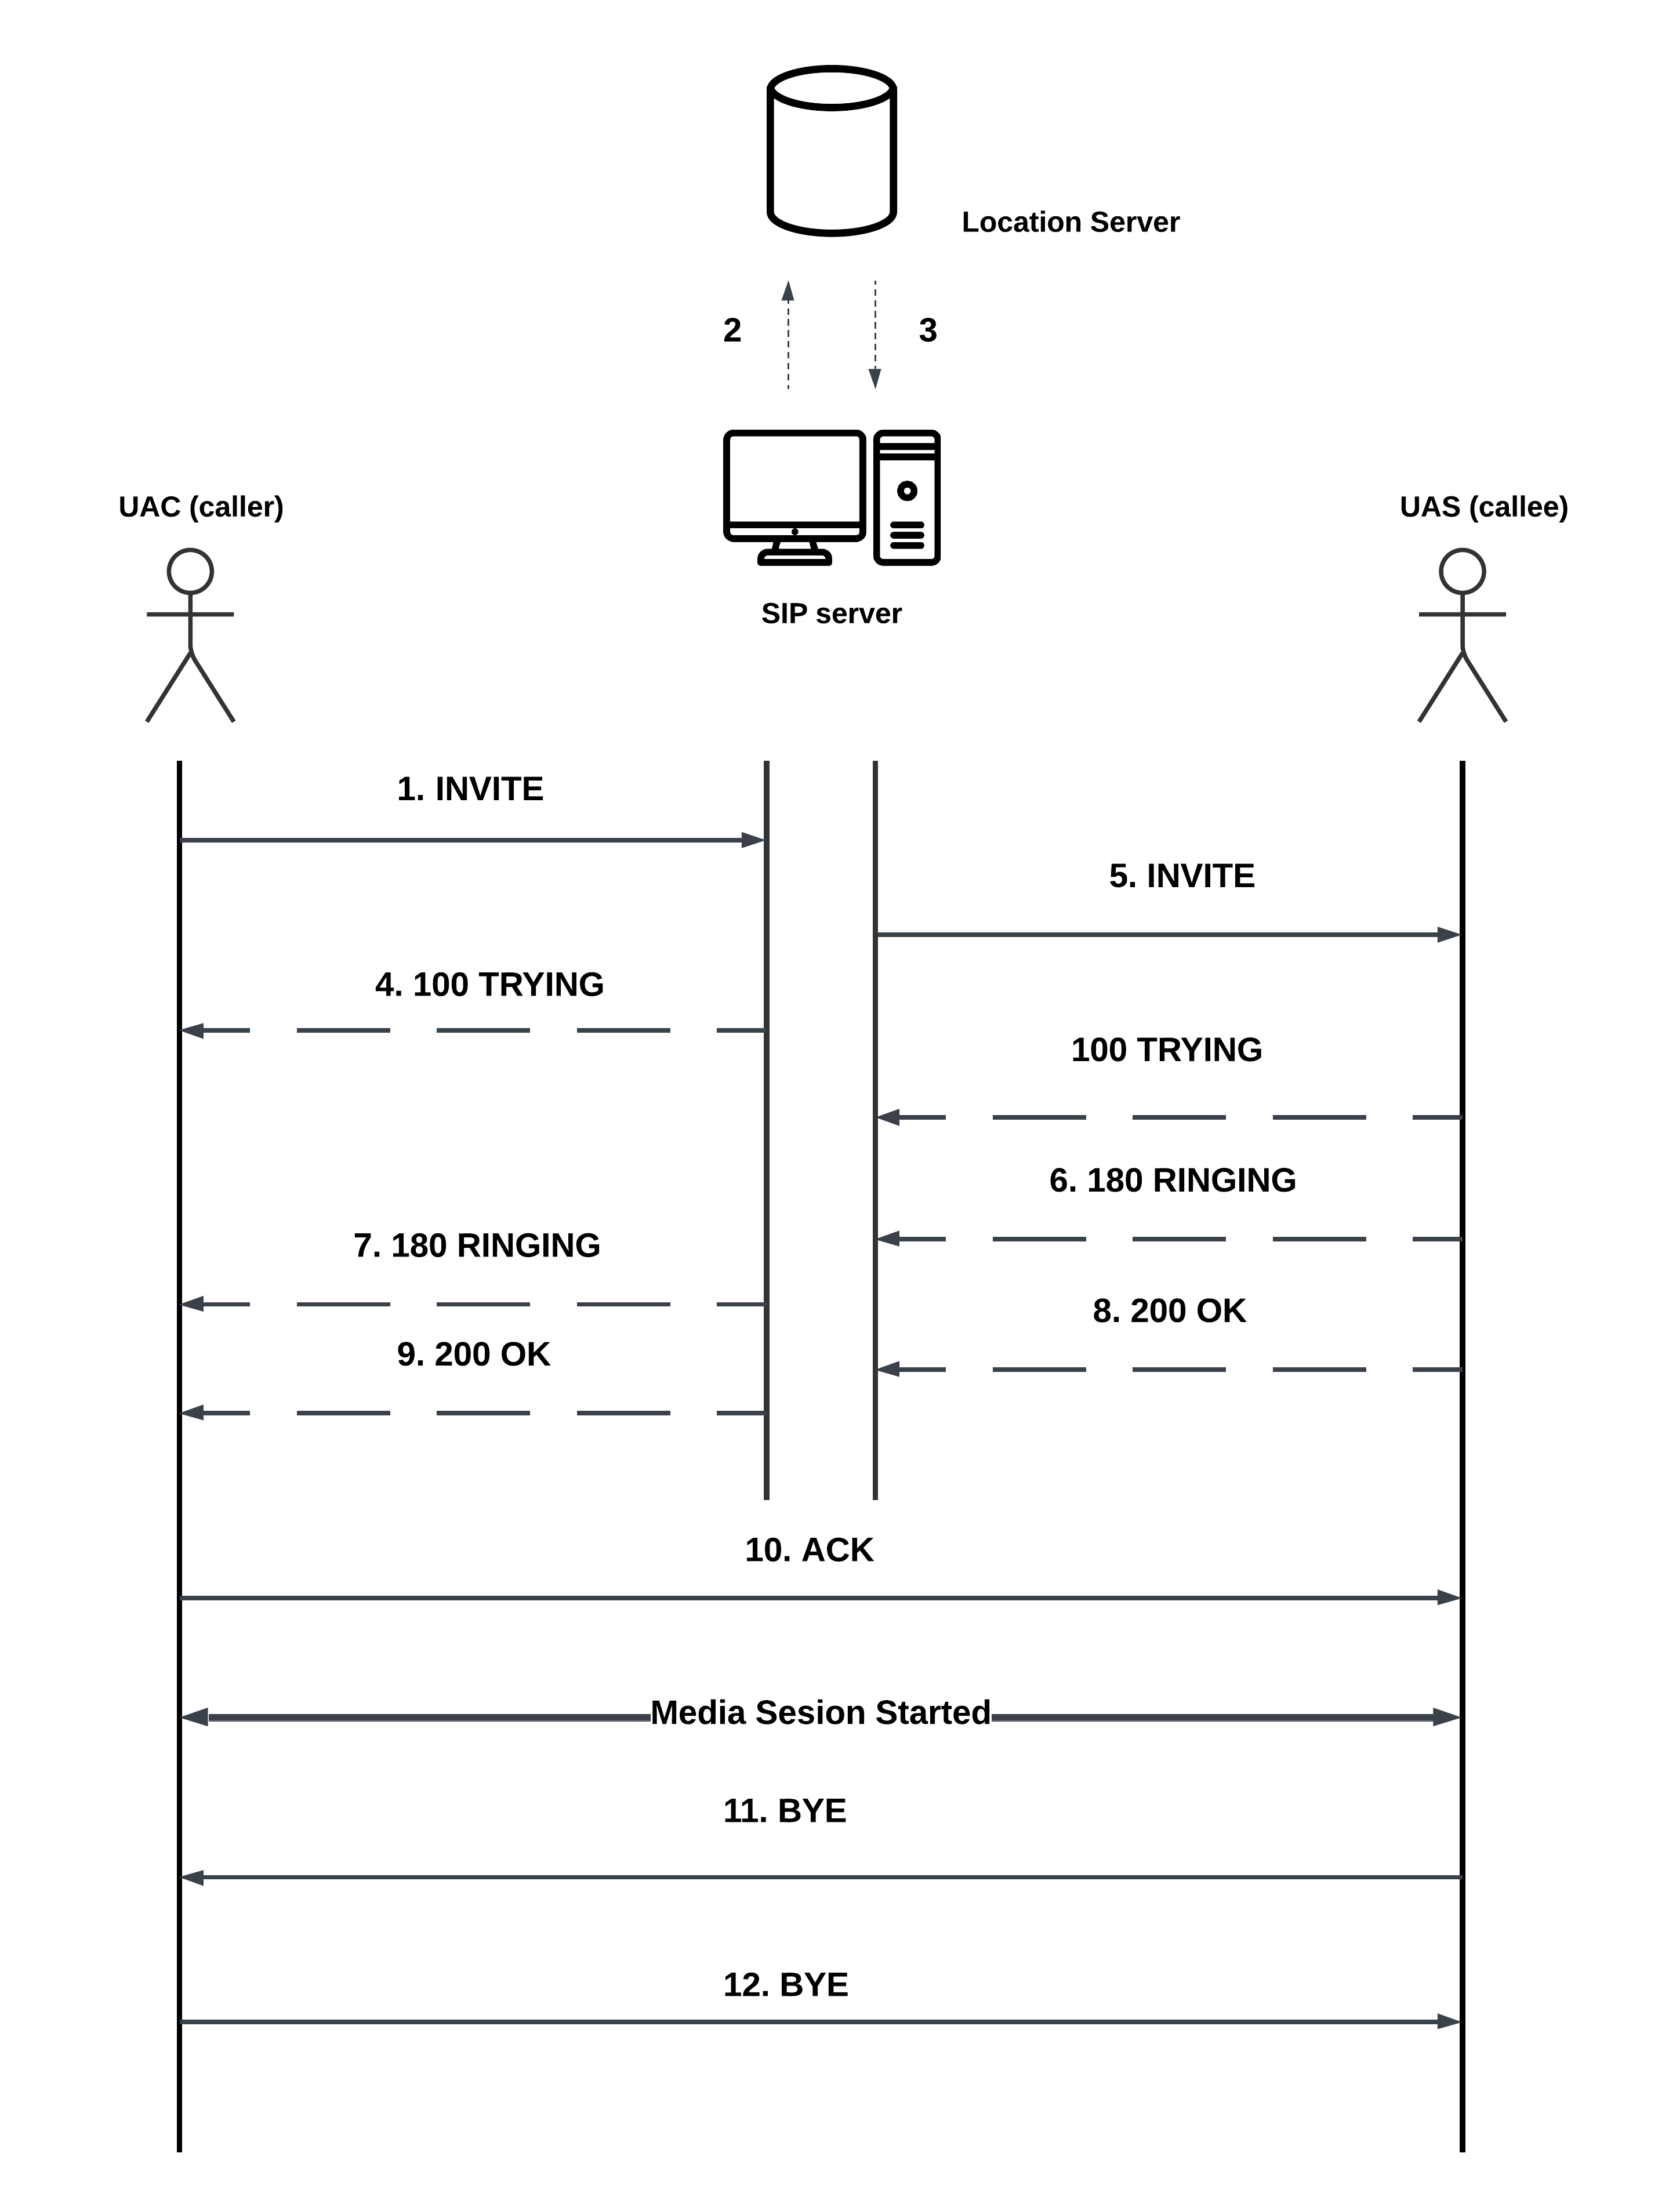
\includegraphics[width=0.7\textwidth]{image/Call Initiation.png} 
        \caption{SIP signaling and key components}
        \label{fig:sip_signaling}
    \end{figure}
    
\subsubsubsubsection{Locating the callee}
    SIP relies on supporting network services like DNS to enable the discovery of proxies and user endpoints. 
    Each user is assigned a unique SIP URI, which is essential for identification and communication. 
    To establish a call using a free SIP service, the following process is typically involved:

    \begin{itemize}
        \item \textbf{Account Registration:} A user registers an account with the free SIP service, which provides a unique SIP URI (e.g., sip: username@sip.linphone.org). 
        This registration associates the user with a proxy server, making them reachable for SIP signaling.
        \item \textbf{Call Setup:} To initiate a call, the SIP client uses the provided SIP URI and sends an INVITE message to the proxy server. 
        The proxy server relies on DNS to locate the callee's proxy server and forwards the INVITE message accordingly.
        \item \textbf{DNS Role in Call Routing:} DNS resolves the domain portion of the SIP URI (e.g., sipserver.com) to the corresponding SIP server's IP address. 
        This process ensures that the caller's proxy server can locate the appropriate next-hop server to route the call.
        \item \textbf{Communication Establishment:}  Once the proxy servers successfully exchange SIP signaling messages, the callee's user agent receives the call request, and the session is established.
    \end{itemize}

    \noindent The figure below shows the SIP registration process and how to detect the location of the callee. 
    \sloppy
    \begin{itemize}
        \item \textbf {Step 1:} One user agent with SIP URI \texttt{sip:callee\_username@sip.linphone.org} register to linphone free sip service registrar server. 
        This server stores the user’s URI and current IP address in its location service database. 
        This makes sure that the user is reachable within the \texttt{sip.linphone.org} domain. 
        \item \textbf {Step 2:} Linphone’s registrar updates its location service with the association of \texttt{sip:\allowbreak callee\_username@sip.linphone.org}.
        \item \textbf {Step 3:} Another user agent (the caller), with the SIP URI \texttt{\allowbreak sip:caller\_username\allowbreak @sip.linphone.org}, 
        sends an INVITE message to their local proxy server. 
        The destination address in the INVITE is \texttt{sip:caller\_username@sip.linphone.org}.
        \item \textbf {Step 4 and 5:} The SIP server will then query for its location service and receive the register address of the callee user agent.
        \item \textbf {Step 6:} The proxy server will then forward the INVITE method to the callee’s device. 
    \end{itemize}

    \begin{figure}[H]
        \centering
        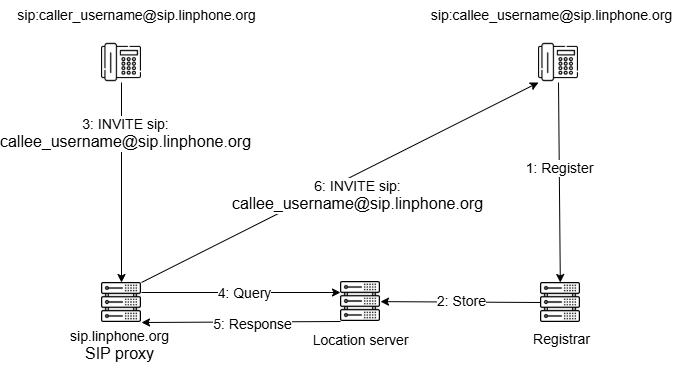
\includegraphics[width=0.7\textwidth]{image/Locating_calllee.png} 
        \caption{SIP registration and locating callee}
        \label{fig:locating_callee}
    \end{figure}

\subsubsubsubsection{One-on-One Instant Messaging}
    Instant Messaging is the process of transfering of messages between users in near real-time.
    The back and forth process to transfer messages have to be fast enough for participants to sustain an interactive dialogue.
    MESSAGE method - an extension to SIP is used to deliver messages between users. 

    \noindent The user must login using the correct right credentials (username and password), that informations will then be send to the Flexisip server of Linphone.
    The Flexisip server will then create a temporary file which includes user contact list information 
% \section{Material and Methodology}
% \subsection{Material}
% \subsubsection{Data Sources}
% In this part we will explain about the process of gathering data
% from scratch, by doing survey.

% \subsubsection{Experimental Setup}
% Still consider what to write for this part. Maybe unecessary.

% \subsection{Methodology}

% This part should describe details the implementation process
% of both mobile development app and machine learning

% Structure: Data describe $\rightarrow$ Mobile app framework $\leftarrow$ Machine Learning Workflow (integrated inside app) $\rightarrow$ Demo for each feature.

% \subsubsection{Mobile App Framework}

% \subsubsection{Machine Learning Workflow}
% In this part, we will describe more detail about:
% \subsubsubsection{Data Preprocessing}

% \begin{itemize}
%     \item describe the data structure
%     \item how and why we using encoding method
%     \item how we split data for training and testing
% \end{itemize}
% \subsubsubsection{Model Configuration and Training}
% In this part we will descrbie detailed about 
% \begin{itemize}
%     \item Model configuration: describe models that we used and why we choose it.
%     \item Model training: process of training the model
% \end{itemize}

% \subsubsubsection{Model Evaluation}
% In this part, we will describe:
% \begin{itemize}
%     \item Attribute we choose to evaluate model performance
%     \item Evaluation metrics: Silhouette score, Davies-Bouldin index
% \end{itemize}

\section{AI Model Analysis and Training}
\subsection{One-Hot Encoding}
One-hot Encoding is a data preprocessing technique that transforms a single categorical variable with n distinct categories 
into n separate columns. Each column is represented by one number 0 or 1, where the value 1 presents the presence of that category 
and the value 0 indicates its absence. This method helps machine learning models, which typically require numerical input, 
better understand and handle the data.

\subsection{Dissimilarity Measure}
The dissimilarity measure between two categorical objects X and Y (with m attributes) can be defined by the total mismatches of their corresponding categorical attributes. The two objects X and Y are considered to be more similar when the value of a mismatched number gets smaller.
        $$d(X,Y) = \sum_{i=1}^{m}\delta{(x_i,y_i)}$$ where $$\delta{(x_i,y_i)} = \left\{\begin{array}{ll} 0 & (x_i = y_i) \\
        1 & (x_i \neq y_i)\end{array}\right.$$

\subsection{K-Mode Algorithm}
% Cost function
Let $\{Q_1,Q_2,...,Q_k\}$ be the modes of clusters $\{C_1,C_2,...,C_k\}$. The cost function can be defined by taking the total dissimilarities of each sample and its assigned cluster's mode: 
$$E = \sum_{l=1}^{k}\sum_{i=1}^{n}y_{i,l}d(X_i,Q_l)$$ 
where $y_{i,l}$ is a binary indicator variable (1 if $X_i$ refers to cluster l, 0 otherwise), k is the number of clusters, n is the total number of samples, $d(X_i,Q_l)$ is the dissimilarity between sample $X_i$ and the mode $Q_l$. The objective is to minimize the value of the cost function by following the following steps: 

\begin{enumerate}
    \item Randomly select K initial modes as K clusters.
    
    \item Calculate the dissimilarity between data points and the mode of each cluster. Then assign objects to the cluster whose mode is closest to it (which has the smallest dissimilarity). Update the cluster’s mode by selecting the highest frequency of each category within the cluster. If there are more than 2 categories of an attribute that have the same highest frequency, we randomly select one of them to serve as mode.
    
    \item Recalculate the dissimilarity of objects with the current modes and reassign the object to the cluster with closest mode and update the new modes for clusters.
    
    \item Repeat Step 2 and 3 until every cluster has no changes after testing the whole dataset.
\end{enumerate}

\subsubsection{Evaluation Metrics}
\paragraph{Silhouette Coefficient}

\paragraph{Davies-Bouldin Index}

\subsection{Model Implementation}

\section{System Design and Implementation}  

\subsection{Hardware and Software Setup}  
This section describes the detailed process of setting up the system, covering hardware and software configurations, as well as initial testing to ensure all components work seamlessly.

\subsubsection{Hardware Setup}  
The essential hardware components for the system include:  
\begin{itemize}  
    \item \textbf{Development Machines: }Computers used for developing and hosting backend services and databases (Spring Boot and PostgreSQL).  
    \item \textbf{User Devices: }Smartphones or virtual devices running the Android app to access features such as Google Calendar, MapBox maps, and Moodle resources.  
    \item \textbf{Networking Equipment: }Tailscale VPN for secure and reliable communication between user devices and the backend server.  
\end{itemize}

\subsubsection{Software Environment Configuration}  
The software setup involves configuring the necessary tools and platforms to support the development and operation of the system:  
\begin{itemize}  
    \item \textbf{Operating System: }Windows was used to host backend services and the database, while Android was the primary platform for the mobile application.  
    \item \textbf{Database: }PostgreSQL was installed and configured as the relational database management system for managing user data, calendar events, location details, and StudyBuddy profiles.  
    \item \textbf{Backend Framework: }Spring Boot was implemented to manage REST API endpoints, handle authentication and authorization, and synchronize data between components.  
    \item \textbf{Mobile Development Tools: }Android Studio served as the primary integrated development environment (IDE) for creating the Android application, leveraging Java and libraries such as Retrofit and MapBox SDK.  
\end{itemize}

\subsection{Application Software}  
The application software comprises several core modules, each designed to handle specific functionalities:  

\begin{itemize}  
    \item \textbf{Authentication and Authorization Module:}  
    \begin{itemize}  
        \item Implements JWT-based authentication.  
        \item Manages Role-Based Access Control (RBAC) for ADMIN and USER roles.  
    \end{itemize}  

    \item \textbf{Google Calendar Integration Module:}  
    \begin{itemize}  
        \item Fetches event data from Google Calendar.  
        \item Detects event updates and sends notifications to the user via the mobile application.  
    \end{itemize}  

    \item \textbf{MapBox Integration Module:}  
    \begin{itemize}  
        \item Stores campus location coordinates (latitude and longitude).  
        \item Dynamically renders campus maps within the app.  
    \end{itemize}  

    \item \textbf{Moodle Resource Module:}  
    \begin{itemize}  
        \item Communicates with Moodle APIs to retrieve course resources, such as slides, source code, and PDFs.  
    \end{itemize}  

    \item \textbf{StudyBuddy Matching Module:}  
    \begin{itemize}  
        \item Collects user profile data (e.g., interests, personality).  
        \item Uses a machine learning recommendation system to suggest matches based on shared interests.  
        \item Features include:  
        \begin{itemize}  
            \item Chat functionality for text-based communication.  
            \item Audio calling capabilities powered by the Linphone library, which provides SIP-based VoIP functionality.  
        \end{itemize}  
    \end{itemize}  

    \item \textbf{Notification System:}  
    \begin{itemize}  
        \item Delivers real-time notifications for calendar updates and incoming calls.  
    \end{itemize}  
\end{itemize}

\subsection{Initial Testing}  
Extensive testing ensured all components functioned correctly and integrated seamlessly:  

\begin{itemize}  
    \item \textbf{Hardware Testing:}  
    \begin{itemize}  
        \item Verified the setup and operation of development machines, servers, and networking equipment using Tailscale VPN for secure communication.  
    \end{itemize}  

    \item \textbf{Software Testing:}  
    \begin{itemize}  
        \item Tested the configuration and performance of the operating system, PostgreSQL database, and Spring Boot services.  
    \end{itemize}  

    \item \textbf{Integration Testing:}  
    \begin{itemize}  
        \item Validated the interaction between backend APIs and mobile app features, ensuring functionality for:  
        \begin{itemize}  
            \item Google Calendar synchronization.  
            \item MapBox map rendering.  
            \item Moodle resource retrieval.  
            \item StudyBuddy matching and chat capabilities.  
            \item Linphone-based audio calling.  
        \end{itemize}  
    \end{itemize}  
\end{itemize}

\subsubsection{Machine Learning Model Integration and Model Training}

This comprehensive setup and testing process ensured that the system was ready for deployment and met the project's objectives effectively.  

\section{Results and Discussion}
\subsection{Results}

\subsubsection{Mobile App Results}
In this part we can have the demo for each feature of the app.

\subsubsection{Machine Learning Results}
In this part we will show the result of the clustering algorithm, using the evaluation 
metrics that we mentioned in the previous section.

\subsection{Discussion}

\section{Conclusion {\&} Future Work}

\subsection{Conclusion}
\subsection{Future Work}



\end{document}

